\documentclass[one column]{report}
\usepackage[utf8]{inputenc}

\usepackage{amsmath,amsthm,amssymb}
\usepackage{mathtools}

\usepackage{subcaption}
\usepackage{graphicx}

\usepackage{comment}

\usepackage{bm}
\renewcommand{\b}[1]{\bm{#1}}
\newcommand{\hatb}[1]{\hat{\b{#1}}}
\newcommand{\tr}{\text{ tr }}
\newcommand{\cov}[2]{\text{cov}(#1,#2)}
\newcommand{\corr}[2]{\text{corr}(#1,#2)}
\newcommand{\mean}[1]{\overline{\b{#1}}}
\usepackage{diagbox}
\newcommand{\abs}[1]{
  \left|
    #1
  \right|}
\newcommand{\rank}[1]{\text{rank #1}}
\newcommand{\diag}{\text{diag }}

\usepackage{biblatex}
\bibliography{ref}

\graphicspath{{./images/}}

\usepackage{listings}


\usepackage{color}

\definecolor{gray}{rgb}{0.5,0.5,0.5}
\definecolor{orange}{rgb}{0.8,0,0}

\lstdefinestyle{matlab}{
  belowcaptionskip=1\baselineskip,
  breaklines=true,
  frame=L,
  xleftmargin=\parindent,
  language=octave,
  showstringspaces=false,
  basicstyle=\footnotesize\ttfamily,
  keywordstyle=\bfseries\color{green},
  commentstyle=\color{gray},
  identifierstyle=\color{blue},
  stringstyle=\color{orange},
}
\lstdefinestyle{R}{
  belowcaptionskip=1\baselineskip,
  breaklines=true,
  frame=L,
  xleftmargin=\parindent,
  language=R,
  showstringspaces=false,
  basicstyle=\footnotesize\ttfamily,
  keywordstyle=\bfseries\color{green},
  commentstyle=\color{gray},
  identifierstyle=\color{blue},
  stringstyle=\color{orange},
}

\def\listingsfont{\ttfamily} 
\def\listingsfontinline{\ttfamily}

\title{TAMS39 - Examination exercises}
\author{Anton Karlsson\\antka388\\931217-7117}
\date{}
\begin{document}
\maketitle

\section*{Exercise 1}

\subsection*{(a)}
\label{sec:a}

Let $H_0: \mu_{\rm female}= \mu_{\rm male}$ against $A \neq H$. The
using Hotelling's $T^2$ test, we find that $H_0$ cannot be rejected in
favor of $A$. Thus we may put $\mu = \mu_{\rm female} = \mu_{\rm male}$.

\subsection*{(b)}
\label{sec:b}

Using \texttt{matlab}, we could plot the confidence ellipse around
${\bf \mu}$, see Figure \ref{fig:ex1-ellipse}.
\begin{figure}[h]
  \centering
  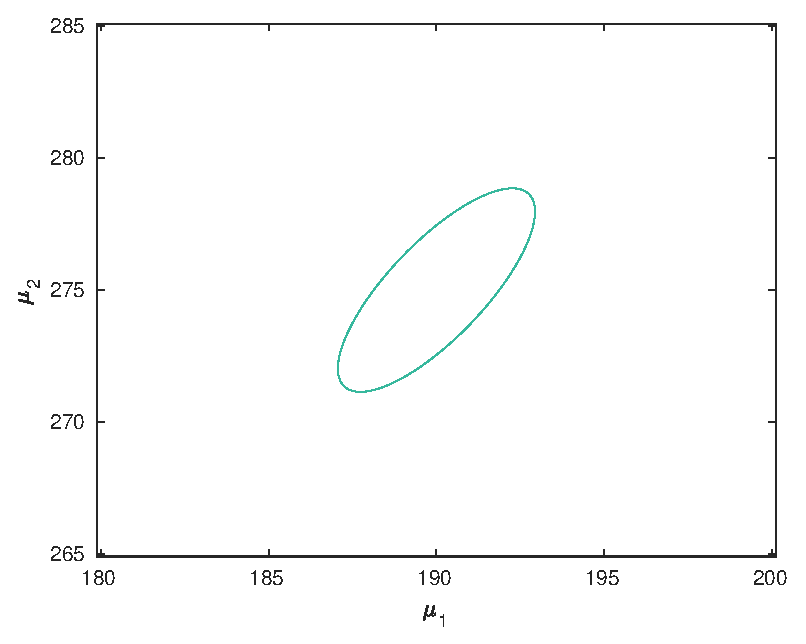
\includegraphics[width=5cm]{ellipse-ex1}
  \caption{The confidence ellipse around ${\bf \mu}$.}
  \label{fig:ex1-ellipse}
\end{figure}

\subsection*{(c)}
\label{sec:c}

Using $a_1 = (1,0)^T$ and $a_2 = (0,1)^T$, we find that the confidence
interval around $\mu_1$ is given by
\begin{equation*}
  \left(
    a \pm T_{1-\alpha} \sqrt{\frac{a_i^T S a_1i^T}{n}}
  \right), \quad i = 1,2,
\end{equation*}
with $T_{1-\alpha} = \frac{n-p}{p(n-1)}F_{1-\alpha}(p, n-p)$. Thus we
get the confidence intervals
\begin{align*}
  (184.7356&,\ 195.2644),\quad i = 1, \\
  (268.0801&,\ 281.9199),\quad i = 2.
\end{align*}


%%% Local Variables:
%%% mode: latex
%%% TeX-master: "examination"
%%% End:


\section*{Exercise 2}
\label{sec:exercise-2}

\subsection*{(a)}
\label{sec:a-1}

The scatter plot can be found in Figure \ref{fig:ex2-scatter} the outlier can be
clearly be seen at $x_1 = 284$.
\begin{figure}[h]
  \centering
  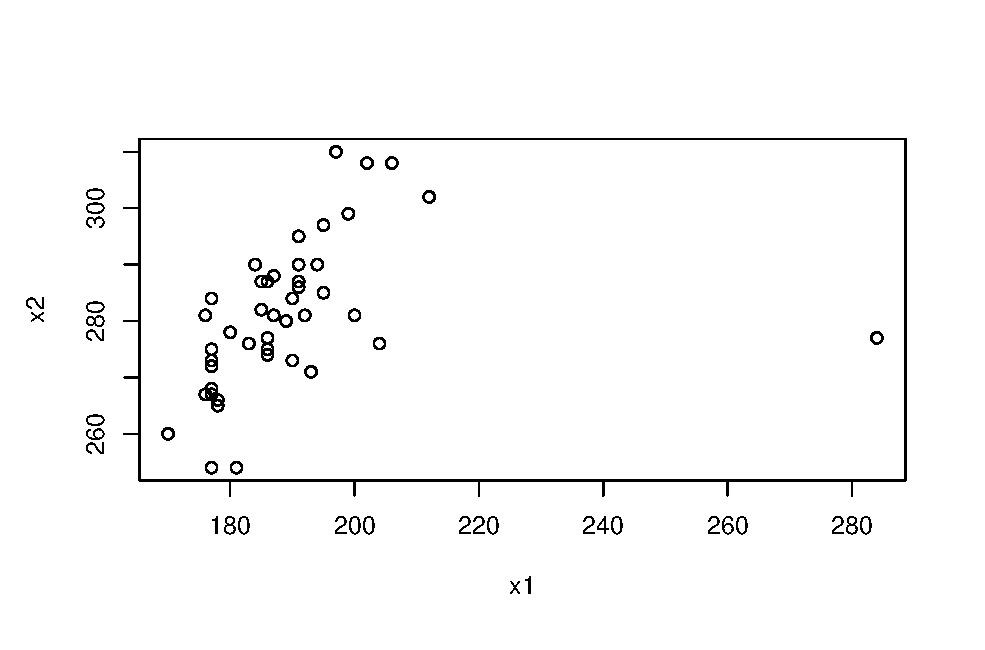
\includegraphics[width=5cm]{ex2-scatterplot}
  \caption{Scatter plot of the tail length and the wing span for male
    hook-billed kites.}
  \label{fig:ex2-scatter}
\end{figure}

\subsection*{(b)}
\label{sec:b-1}

Using the Box corrected test found in \cite[p. 311]{book}, we find that
we can not pool the covariance matrices (see code for details).

\subsection*{(c)}
\label{sec:c-1}

In this test, the pooled matrix $S_p$ was used. Using the Hotelling's
$T^2$ test, we can put $\delta = \bar{x}_{\rm male}- \bar{x}_{\rm
  female}$, we can use the test variable
\begin{equation*}
  T^2 = \frac{n_{\rm female}  n_{\rm male}}{n_{\rm female} +  n_{\rm male}}\delta^T S_p^{-1}\delta,
  \label{eq:1}
\end{equation*}
and rejected $H_0: \mu_{\rm male} = \mu_{\rm female}$ if the test
variable is larger than
\begin{equation*}
 c  = \frac{fp}{f-p+1}F_{1-\alpha}(p, n-p), %c = f*p*qf(1-0.05, p, f-p)/(f-p+1)
\end{equation*}
where $f = n - 1$, and $p = 2$. Since $T^2 = 7.494772$ and $c =
6.27986$, we reject $H_0: \mu_{\rm male} = \mu_{\rm female} $.

The result would most likely hold if we changed the value of the
outlier to $x_1 = 184$ instead of 284, since the sample size should be too
large enough for any drastic changes in the variance matrix or mean to
happen.

\subsection*{(d)}
\label{sec:d}
??

\subsection*{(e)}
\label{sec:e}

The confidence region if given by the equation, for $\mu = (\mu_1, \mu_2).$
\begin{equation}
  \label{eq:ex2-conf-region}
 \{\mu:\ n (\delta - \mu)^T S_p^{-1} (\delta-\mu)\leq \frac{(n-1)p}{n-p}F_{1-\alpha}(p,n-p)\},
\end{equation}
where $\alpha = 0.05$, $S_p$ is the pooled matrix from the previous
exercise, and $\delta = \bar{x}_{\rm male}  - \bar{x}_{\rm
  female}$. Computing the LHS of \eqref{eq:ex2-conf-region}, get
\begin{align*}
  89
  \big(
    &206.7294 ( - 6.463131 -\mu_1)^2 + 189.1233(1.176768 -\mu_2)^2 \\
    &+ 202.2905(- 6.463131 - \mu_1)(1.176768- \mu_2)
  \big)\\
  &\leq \frac{88\cdot 2}{87}3.103839
\end{align*}
Further, to find the confidence intervals for the the different
components, we use the vectors $a_1 = (1,0)^T$ and $a_2 = (0,1)^T$, to
create each of the component wise intervals, respectively. The
intervals, for each $a$, is given by 
\begin{equation*}
  n_f n_m \delta^T S_p^{-1} \delta / (n_f + n_m) , 
\end{equation*}
where.
we get the intervals
\begin{align*}
  (-170.698117786475&; 157.771855160212), \quad \text{for } a = (1,0)
  \\
  (-149.071120157853&;151.424655511388), \quad \text{for } a = (0,1)
\end{align*}

\subsection*{(f)}
\label{sec:f}

From the interval we find the Exercise (e), we see that there are no
genrall difference for the lengths between the female and the male birds.
\subsection*{\texttt{R} code}
\label{sec:textttr-code}

\lstinputlisting[style=R]{../ex2.R}

%%% Local Variables:
%%% mode: latex
%%% TeX-master: "examination"
%%% End:

\section*{Exercise 3}
\label{sec:exercise-3}

\subsection*{(a)}
\label{sec:a-2}
The plot of the profiles are presented in figure
\ref{fig:ex3-profiles}.
\begin{figure}[h]
  \centering
  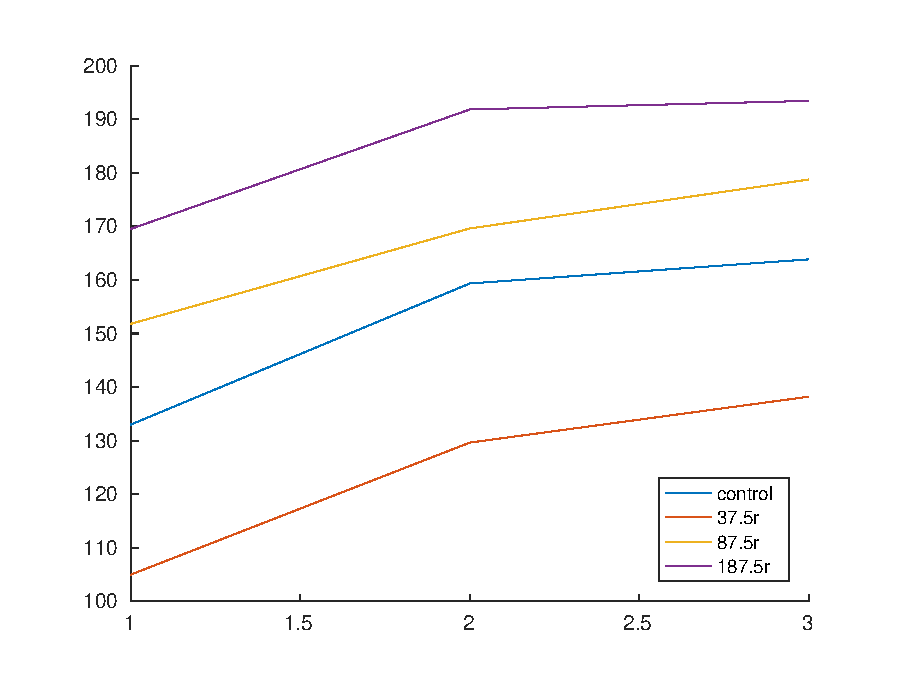
\includegraphics[width=8.5cm]{ex3-profiles}
  \caption{The profiles for the Psychomotor scores given different
    radiation treatment.}
  \label{fig:ex3-profiles}
\end{figure}

\subsection*{(b)}
\label{sec:b-2}

%Check the updated code, which should probably correct. 

To test if the profiles are parallel the test presented in Lecture
7 is used. First we introduce the matrices
\begin{align*}
  \b A &=
         \begin{pmatrix}
           \b 1_{n_{1}}  & \b 0_{n_{1}}& \b 0_{n_{1}}& \b 0_{n_{1}} \\
           \b 0_{n_{2}} &  \b 1_{n_{2}}  &\b 0_{n_{2}}& \b 0_{n_{2}} \\
           \b 0_{n_{3}}& \b 0_{n_{3}}&  \b 1_{n_{3}}  & \b 0_{n_{3}} \\
           \b 0_{n_{4}}& \b 0_{n_{4}}& \b 0_{n_{4}} &   \b 1_{n_{4}}   \\ 
         \end{pmatrix} \\
  \b V &= \b X^{T} (\b I_{n}   -  \b A(\b A^{T}\b A)^{-1}\b A^{T}) \b X, \\
  \b C &=
         \begin{pmatrix}
           1 & -1 & 0 \\
           1 &  0 & -1
         \end{pmatrix}, \\
  \b Y &=
         \begin{pmatrix}
           \b \mu_{1} - \mu_{4} &\b \mu_{2} - \mu_{4} &\b \mu_{3} - \mu_{4} 
         \end{pmatrix} \\
  \b C_{Y}^{-1} &= \diag (n_{1}, n_{2}, n_{3}) - \frac{1}{n}   (n_{1},
                  n_{2}, n_{3})^{T} (n_{1}, n_{2}, n_{3}), \\
  \b H &= \b Y\b C_{Y}^{-1}\b Y^{T}                  
\end{align*}
Then we construct the test statistic
\begin{equation*}
  Q = -
  \left(
    n - \frac{1}{2}(k + p + 1)
  \right)
  \left(
    \ln \abs{\b {CVC}^{T}} - \ln \abs{\b{CVC}^{T} + \b{CHC}^{T}}
  \right) ,
\end{equation*}
where we reject $H_{1}: $ \textit{the profiles are parallel} if $Q$ is larger
than 
\begin{equation*}
  c = \chi^{2}_{(p-1)(k-1)}(1 - \alpha), \quad \alpha = 0.05.
\end{equation*}
Since $Q =4.0443 $ and $c = 12.5916$, we cannot reject $H_{1}$, the
profiles are parallel


\subsection*{(c)}
\label{sec:c-2}

Since, the profiles are parallel, we can set up a test for checking if
the profiles are on the same level. The likelihood ratio is 
\begin{equation*}
  \lambda_{H_2 | H_1} = \frac{\abs{\b C\b V \b C^{T} + \b C \b H\b C^T}}{\abs{\b
      C\b V \b C^T}}\frac{\abs{\b V}}{\abs{\b V+\b H}},
\end{equation*}
from which $H_{2}|H_{1}$ is rejected if 
\begin{equation*}
  Q = \left(\frac{n-k - p +1}{k - 1}\right)\frac{1 - \lambda_{H_2 |H_1}}{\lambda_{H_2 | H_1}},
\end{equation*}
is larger then 
\begin{equation*}
  c = F_{k-1, n - k - p +1} (1 - \alpha), \quad \alpha = 0.05
\end{equation*}
We get
\begin{equation*}
 7.9361  = Q < c = 3.2145,
\end{equation*}
so $H_2 | H_1$ is rejected, the profiles are not on the same level.

\subsection*{(d)}
\label{sec:d-1}

Here, we use the test variables 
\begin{equation*}
  \lambda_{H_3 | H_1} = \frac{1}{1 + n \bar{\bf x}^T \b C^T (\b{CVC}^T +
    \b{CHC}^T)^{-1}}\b C\bar{\bf x},
\end{equation*}
and create the test variable
\begin{equation*}
  Q = \frac{n - p +1}{p - 1}\lambda_{H_3 |H_1}, 
\end{equation*}
which we compare to 
\begin{equation*}
  c = F_{p-1, n-p+1}(0.95).
\end{equation*}
We get
\begin{equation*}
  7.9361 = Q > c = 3.2145.
\end{equation*}
Thus $H_3 | H_1$ is rejected, the profiles are not flat.
%%% Local Variables:
%%% mode: latex
%%% TeX-master: "examination"
%%% End:

\section*{Exercise 4}
\label{sec:exercise-4}

\subsection*{(a)}
\label{sec:a-3}

To check if the covariance matrices can be pooled, the hypothesis
$H_{0}: \Sigma_{1} =\Sigma_{2}  = \Sigma_{3}$ is considered. We
reject $H_{0}$ if
\begin{equation*}
  \Lambda^* = \frac{\prod_{i = 1}^{3} \abs{\b V_i}^{f_i/2}}{\abs{\b V}^{f/2}}
  \frac{f^{pf/2}}{\prod_{i = 1}^{3} f_i ^{pf_{i}/2}} < c,\quad
  \text{for some } c,
\end{equation*}
where $f_{i} = n_{i} - 1$, are the degrees of freedom for group $i = 1,
2, 3$, $f = \sum_{i=1}^{3}f_{i}$, and
\begin{equation*}
  \b V_{i} = \b X_{i} (\b I_{n_{i}}  - \frac 1n_{i}\b 1_{n_{i}} \b 1_{n_{i}}^{T})^{T}
  \b X_{i}^{T},\quad i = 1,2,3,
\end{equation*}
and
\begin{equation*}
  \b V = \sum_{i=1}^{3} \b V_{i}.
\end{equation*}
The test $\Lambda^{*} < c$, for some $c$, is an unbiased test.
Further, we can use the correction found in Lecture 5, where
\begin{equation*}
  -2 \frac{m}{f} \ln \Lambda^{*} \sim \chi^{2}(df), \quad df = \frac{1}{2}p(p+1)(r-1),
\end{equation*}
where $m = f- 2\alpha$, where
\begin{equation*}
  \alpha = 
  \left(
    \sum_{i = 1}^{3} \frac{f}{f_{i}} - 1
  \right)
  \frac{2p^{2} + p -1}{12(p+1)(3-1)}.
\end{equation*}
Then 
\begin{equation*}
   -2 \frac{m}{f} \ln \Lambda^{*} = 49.26
\end{equation*}
and
\begin{equation*}
  \chi_{df}^{2}(1-\alpha) = 91.670, \quad \alpha = 0.05,
\end{equation*}
hence $H_{0}$ cannot be rejected, the covariance matrices can be
pooled. 
\subsection*{(b)}
\label{sec:b-3}

Since we can pool the sample matrix, which is given as
\begin{equation*}
  \b S_{\rm spooled} =
  \begin{pmatrix}
    156.82 &57.13 &20.27 &22.13 &0.16 &20.40 \\ 
    57.13 &53.20 &10.93 &9.57 &-0.47 &11.67 \\ 
    20.27 &10.93 &5.95 &6.30 &-0.23 &4.67 \\ 
    22.13 &9.57 &6.30 &22.39 &-0.54 &11.37 \\ 
    0.16 &-0.47 &-0.23 &-0.54 &0.99 &0.06 \\ 
    20.40 &11.67 &4.67 &11.37 &0.06 &53.09 
  \end{pmatrix},
\end{equation*}
we can use the distance function $d_{i}(\b x_{0}) = (\b x_{0} - \mean
x_{i})^{T} \b S_{\rm spooled}^{-1} (\b x_{0} - \mean
x_{i})$ given in \cite[p. 611]{book}, where  $\b x_{0}$ is classified to
$\pi_{i}$ if $d_{i}(\b x_{0}) = \min_{i = 1, 2, 3}
\left\{
    d_{i}(\b x_{0})
\right\}$. The distance functions can be created with
\begin{equation*}
  S_{\rm pooled}^{-1} =
  \begin{pmatrix}
    0.01 &-0.01 &-0.03 &-0.00 &-0.01 &-0.00 \\ 
    -0.01 &0.04 &-0.04 &0.01 &0.01 &-0.00 \\ 
    -0.03 &-0.04 &0.42 &-0.07 &0.04 &-0.00 \\ 
    -0.00 &0.01 &-0.07 &0.07 &0.03 &-0.01 \\ 
    -0.01 &0.01 &0.04 &0.03 &1.05 &-0.01 \\ 
    -0.00 &-0.00 &-0.00 &-0.01 &-0.01 &0.02  
  \end{pmatrix},
\end{equation*}
and 
\begin{equation*}
  \mean x_{1} =
  \begin{pmatrix}
    183.10 \\ 
    129.62 \\ 
    51.24 \\ 
    146.19 \\ 
    14.10 \\ 
    104.86 
  \end{pmatrix}, \quad 
  \mean x_{2} =
  \begin{pmatrix}
    201.00 \\ 
    119.32 \\ 
    48.87 \\ 
    124.65 \\ 
    14.29 \\ 
    81.00  
  \end{pmatrix}, \quad 
  \mean x_{3} =
  \begin{pmatrix}
    138.23 \\ 
    125.09 \\ 
    51.59 \\ 
    138.27 \\ 
    10.09 \\ 
    106.59
  \end{pmatrix}.
\end{equation*}



\subsection*{(c)}
\label{sec:c-3}
Since both the means and the varaince is unkown, we use the estimates
of the errors of missclassification according to Okamato. First define 
\begin{align*}
  a_{1} &= \frac{\hat\Delta^{2} +
    12(p-1)}{16\hat\Delta}\phi(\hat\Delta) =0.99 ,  \quad a_{2} =
  \frac{\hat\Delta^{2} + 4(p-1)}{16\hat\Delta}\phi(\hat\Delta) =0.18 , \quad
  \text{and}\quad \\
  a_{3} &= \frac{\hat\Delta(p-1)}{4}\phi(\hat\Delta) = 7.70,
\end{align*}
where 
\begin{equation*}
  \hat\Delta^{2} = \frac{f - p - 1}{f} (\mean x_{1} - \mean x_{2})^{T}
  \b S_{\rm pooled}^{-1} (\mean x_{1} - \mean x_{2}) = 6.16,
  \quad f = n_{1} + n_{2} - 2 = 50.
\end{equation*}
Then the error of missclassificating a member of $\pi_{0}$ onto 
$\pi_{1}$ is given by 
\begin{equation*}
  e_{1} = P(\b x_{0} \in \pi_{2}) \approx  \phi(-\frac 12 \hat\Delta) + \frac{a_{1}}{n_{1}} +
  \frac{a_{2}}{n_{2}} + \frac{a_{3}}{f} = 0.21,  
\end{equation*}
and the error of missclassificating a member of $\pi_{0}$ onto 
$\pi_{2}$ is
\begin{equation*}
  e_{1} = P(\b x_{0} \in \pi_{1}) \approx  \phi(-\frac 12 \hat\Delta) + \frac{a_{2}}{n_{1}} +
  \frac{a_{1}}{n_{2}} + \frac{a_{3}}{f} = 0.20.
\end{equation*}

%%% Local Variables:
%%% mode: latex
%%% TeX-master: "examination"
%%% End:


\begin{comment}
  
  We could calculate the linear separators, $ l_i^T x_0 + c_i$, where
  we obtain
  \begin{align*}
    l_1^T x_0 + c_1 &= (-0.57, 1.80, 1.01, 6.33, 18.94, 0.33)x_0 + -703.95 \\ 
    l_2^T x_0 + c_2 &= (-0.14, 1.31, 1.48, 5.15, 18.31, 0.04)x_0 + -554.06 \\ 
    l_3^T x_0 + c_3 &= (-1.08, 1.89, 3.03, 5.69, 15.11, 0.51)x_0 + -618.43,
  \end{align*}
  In which we can conclude that ${\bf x_0}$ belongs to  $\pi_i$ if $
  l_i^T x_0 + c_i = \max_i \left(   l_i^T x_0 + c_i\right)
  $

\end{comment}

\section*{Exercise 5}
\label{sec:exercise5}

\subsection*{(a)}
\label{sec:a-4}

The dot diagrams\footnote{Jag är lite osäker på hur dot diagram ska se
  ut. Och framföralt hur man gjorde ett i \texttt{matlab}, men jag
  hoppas att detta illusterar det du är ute efter.} are shown in Figure \ref{fig:ex5-marginalplots}. 

\begin{figure}[h]
  \centering
  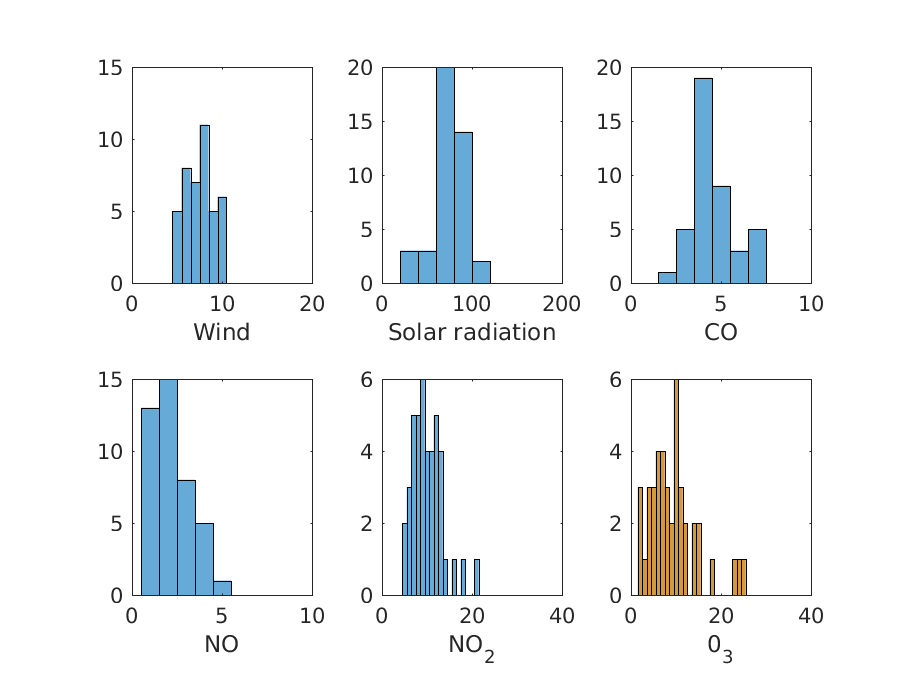
\includegraphics[width=13cm]{ex5-marginalplots}
  \caption{The marginal dot diagrams for all variables}
  \label{fig:ex5-marginalplots}
\end{figure}

\subsection*{(b)}
\label{sec:b-4}

The sample mean is given as
\begin{equation*}
  \bar{x} =
  \begin{pmatrix}
    7.50 & 73.86 & 4.55 & 2.19 & 10.05 & 9.40 & 3.10 
  \end{pmatrix}^T
\end{equation*}
and
\begin{equation*}
  S =
  \begin{pmatrix}
    2.50 & -2.78 & -0.38 & -0.46 & -0.59 & -2.23 & 0.17 \\ 
    -2.78 & 300.52 & 3.91 & -1.39 & 6.76 & 30.79 & 0.62 \\ 
    -0.38 & 3.91 & 1.52 & 0.67 & 2.31 & 2.82 & 0.14 \\ 
    -0.46 & -1.39 & 0.67 & 1.18 & 1.09 & -0.81 & 0.18 \\ 
    -0.59 & 6.76 & 2.31 & 1.09 & 11.36 & 3.13 & 1.04 \\ 
    -2.23 & 30.79 & 2.82 & -0.81 & 3.13 & 30.98 & 0.59 \\ 
    0.17 & 0.62 & 0.14 & 0.18 & 1.04 & 0.59 & 0.48 \\ 
  \end{pmatrix}
\end{equation*}

\subsection*{(c)}
\label{sec:c-4}

The model used was
\begin{equation*}
  y_1 = \beta_0 + \beta_1 x_1 + \beta_2 x_2 + \epsilon,
\end{equation*}
where $\hat{\beta} = (10.1145,\   -0.2113,\    0.0205)$. From here we
can calculate the residual:
\begin{equation*}
  \text{SS}_{\rm E} = 455.1356.
\end{equation*}

Further, we got the following confidence interval with confidence level of 95
\%: $(7.59, 11.71)$. 

\subsection*{(d)}

Here, we propose the linear model
\begin{equation*}
  \begin{pmatrix}
    y_1 \\ y_2
  \end{pmatrix} = 
  BX + E,
\end{equation*}
where 
\begin{equation*}
  X =
  \begin{pmatrix}
    {\bf 1_n} & x_2 & x_2
  \end{pmatrix}.
\end{equation*}
We found that
\begin{equation*}
  B =
  \begin{pmatrix}
    10.11 & -0.21 \\ 
    0.02 & 8.28 \\ 
    -0.79 & 0.10 
  \end{pmatrix}.
\end{equation*}

The confidence region for $x_1 = 10$ and $x_2 = 80$ is shown in Figure
\ref{fig:ex5-ellipse}
\begin{figure}[h]
  \centering
  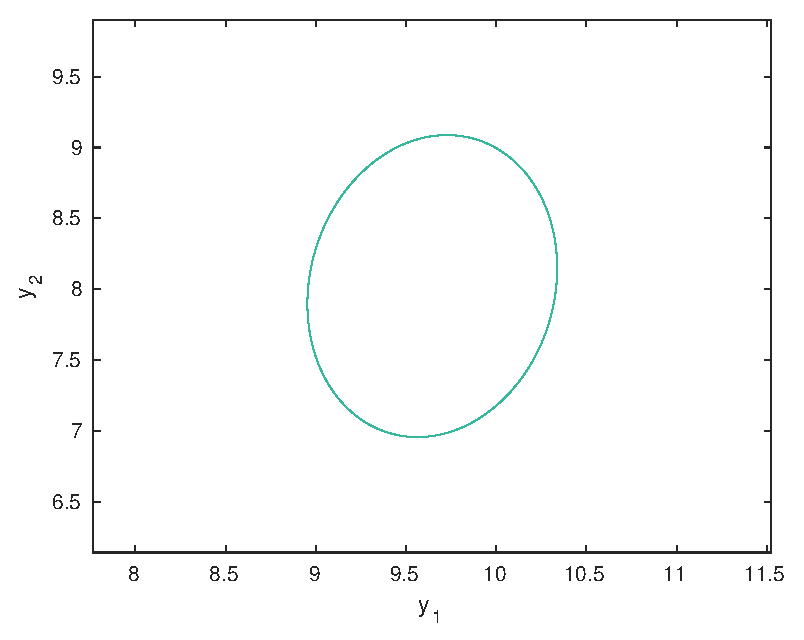
\includegraphics[width=7cm]{ex5-ellipse}
  \caption{The confidence region for $x_1 = 10$ and $x_2 = 80$. }
  \label{fig:ex5-ellipse}
\end{figure}

We can see that the ellipse is covered by 
the confidence interval in Exercise~(c), on the $y_1$ axis.

%%% Local Variables:
%%% mode: latex
%%% TeX-master: "examination"
%%% End:


\section*{Exercise 6}
\label{sec:exercise-6}

\subsection*{(a)}
\label{sec:a-5}


The foll wing linear model was designed
\begin{equation*}
  \b Y = \b{XB},
\end{equation*}
where $\b Y$ is the out parameters and $\b X$ is the design matrix
\begin{equation*}
  \b X = (\b 1_n, \b x_1, \b x_2),
\end{equation*}
and $\b B:(3 \times 4) $ contained the unknown parameter values, which
was estimated using linear regression as
\begin{equation*}
  \b B =
  \begin{pmatrix}
    -94.60 &-228.67 &-258.80 &-246.05 &-232.96 \\ 
    19.27 &43.65 &48.99 &47.33 &45.10 \\ 
    -24.68 &-20.59 &3.32 &5.22 &8.24 
  \end{pmatrix}.
\end{equation*}

\subsection*{(b)}
The sample correlation matrix was 
\begin{equation*}
  \b R =
  \begin{pmatrix}
    1.00 &0.86 &0.71 &0.64 &0.65 &0.81 &-0.09 \\ 
    0.86 &1.00 &0.91 &0.89 &0.90 &0.95 &0.10 \\ 
    0.71 &0.91 &1.00 &0.98 &0.98 &0.92 &0.22 \\ 
    0.64 &0.89 &0.98 &1.00 &1.00 &0.90 &0.22 \\ 
    0.65 &0.90 &0.98 &1.00 &1.00 &0.90 &0.24 \\ 
    0.81 &0.95 &0.92 &0.90 &0.90 &1.00 &0.22 \\ 
    -0.09 &0.10 &0.22 &0.22 &0.24 &0.22 &1.00  
  \end{pmatrix}.
\end{equation*}
was is interesting is that the time steps that are close to each other
correlates more than those times further apart. We can even note that
the first and last time steps have negative correlation an is almost 0.

\subsection*{(c)}
\label{sec:c-5}

We can the test if the \textit{average weight} affect the causation of
death by considering the test where each element of the bottom row of $\b
B$ should be equal to zero. We get the hypothesis
\begin{equation*}
  H_0:\ \b{CB} = \b 0,
\end{equation*}
where 
\begin{equation*}
  C = 
  \begin{pmatrix}
    0 &0 &0 \\ 
    0 &0 &0 \\ 
    0 &0 &0 \\ 
    0 &0 &0 \\ 
    0 &0 &1   
  \end{pmatrix},
\end{equation*}
form which could use the test described on page 11 of Lecture 9, and use
the corresponding asymptotic expansion found on page 12 of Lecture 9 to
test on a significance level of 5 \%. We find that 
\begin{align*}
  p &= P(\chi^2 \geq z) + (\gamma/\nu^2)P(\chi^2 \geq z) -  P(\chi^2
      \geq z )\\
    &\approx 0.7931 > 0.05,
\end{align*}
hence we reject $H_0$.
%%% Local Variables:
%%% mode: latex
%%% TeX-master: "examination"
%%% End:


\subsection*{Exercise 7}
\label{sec:exercise-7}

Since there are no structure for the mean, the sample covariance matrix
is created by taking the sample covariance matrix of $\b X = [X_{1},
X_{2}, X_{3}, X_{4}]$ with dimension $(n \times p)$, where $n = 45$ and
$p= 11$, and the matrices $X_{i}$ represents the samples of the
different groups. We let $i = 1$ be the control group, $i = 2$ be
25-50r, $i = 3$ be 75-100r, and $i = 4$ be  125-250r. \\
\\
The hypothesis $H_{0}: \b\Sigma = \sigma^{2}[(1-\rho)\b I + \rho \b 1
\b 1^{T}]$ is not rejected if
\begin{equation*}
  \left[ n  - 1 - \frac{p(p+1)^2 (2p-3)}{6(p-1)(p^2+p-4)} \right] \ln
    \Lambda < \chi^{2}_{g}(0.95),
\end{equation*}
where 
\begin{equation*}
  g = \frac{1}{2}p(p+1) -2 = 64,
\end{equation*}
and
\begin{equation*}
 \ln\Lambda = \ln\abs S- \ln\frac{\b 1^{T} \b S \b 1}{p}  - (p-1)\ln\frac{p\tr S - \b 1^{T} \b S \b 1}{p(p-1)}.
\end{equation*}
We get that
\begin{equation*}
  \left[ n  - 1 - \frac{p(p+1)^2 (2p-3)}{6(p-1)(p^2+p-4)} \right] \ln
    \Lambda \approx 263.05,
\end{equation*}
which is larger than
\begin{equation*}
  \chi^{2}_{g}(0.95) \approx 83.68.
\end{equation*}
So $H_{0}$ is rejected, there are no intraclass covariance matrix.

\subsection*{(b)}
\label{sec:b-6}

Further, we which to test if the correlation matrix is zero on all the
sub diagonals. We use the test found in Exercise 8.9 from \cite[p. 472]{book}. Set 
\begin{equation*}
  \ln \Lambda = \frac n2 \ln |\b S |- \frac n2 \sum_{i = 1}^{p} \ln\b (S_{ii}),
\end{equation*}
and 
\begin{equation*}
  u = 2\left(1 - \frac{2p + 11}{6n}\right).
\end{equation*}
We find that that the test size
\begin{equation*}
  -u \ln \Lambda = 1159.79  > 73.31 = c = \chi^2_{p(p-1)/2}(0.95).
\end{equation*}
Thus, it can be concluded that the scores at each time step is not
independent. 

\subsection*{(c)}
\label{sec:c-6}

We consider the growth curve model 
\begin{equation*}
  \b Y = \b{ABC} +  \b E,
\end{equation*}
where $A = (\b 1_{p},\b t)$, $\b t = (0, 1, \dots, p - 1)^{T}$, $p =
10$,  $\b B$ contains
the parametric values, where each column 
consist of the parametric values for each group,  and $\b C$ is a
matrix of controlling which group each column in $\b B$ belong to. The
matrix $\b E \sim N_{p, n}(\b 0, \b \Sigma, \b I)$. We can write $\b C$ as
\begin{equation*}
  \b C =
  \begin{pmatrix}
    \b 1_{n_{1}}^{T} & \b 0_{n_{2}}^{T} & \cdots & \b 0_{n_{k}}^{T} \\
    \b 0_{n_{1}}^{T} & \b 1_{n_{2}}^{T} & \cdots & \b 0_{n_{k}}^{T} \\
    \b 0_{n_{1}}^{T} & \b 0_{n_{2}}^{T} & \cdots & \b 1_{n_{k}}^{T}
  \end{pmatrix},
\end{equation*}
where $k = 4$ is the number of groups. \\
\\
The solution of finding the parameters in $\b B$ is given by 
\begin{align*}
  \b \hat B &= (\b A^{T}\b V^{-1}\b A)^{-1}  \b A^{T}\b V^{-1}\b Y
              \b C^{T}(\b C\b C^{T})^{-1} % looks great!
  \\
  &=
  \begin{pmatrix}
    117.39 &96.64 &121.25 &150.95 \\ 
    7.38 &5.43 &5.11 &5.34
  \end{pmatrix},
\end{align*}
where
\begin{equation*}
  \b V =  \b Y  (\b I - \b P_{c})  \b Y^{T},
\end{equation*}
where
\begin{equation*}
  \b P_{c} = \b C^{T}(\b C\b C^{T})^{-1}\b C.
\end{equation*}
% The oter matrices are to large to be displayed here. 

\subsection*{(d)}
\label{sec:d-2}

To compare the parameters we consider three different tests,
\begin{equation*}
  H_i: \b B^{(1)} - \b B^{(i)} = \b 0,\quad i = 2,3,4,
\end{equation*}
where $\b B^{(i)}$ denotes column $i$ of $\b B$. We can reformulate the
hypothesis $i$ as
\begin{equation*}
  H_i: \b{G B H_i} = \b 0, \quad i = 2,3,4,
\end{equation*}
where the matrix $\b H_i$ has its first element equal to 1 and its $i$th element
equal to $-1$. The matrix $\b G$ is just the identity matrix of
dimension 2. We reject $H_{i}$ if 
\begin{equation*}
  \Lambda_{i} = \frac{\abs{\b G (\b A^{T} \b V^{-1} \b A)^{-1}\b G^{T}}}
  {\abs{\b G (\b A^{T} \b V^{-1} \b A)^{-1} \b G ^{T} + \b G \b \hat B\b H_{i}(\b
      H_{i}^{T} \b R \b H_{i})^{-1}\b H_{i}^{T} \b \hat B^{T} \b G^{T}}}
\end{equation*}
where
\begin{align*}
  \b R = (\b C \b C^{T})^{-1} + ( &\b C \b C^{T})^{-1} CY^{T} \\
 &  \cdot\left[
    \b V^{-1}  - \b V^{-1}\b A(\b A^{T} \b V^{-1} \b A)^{-1}\b A^{T} \b V^{-1}
  \right] 
  \b Y \b C^{T}(\b C \b C^{T})^{-1}.
\end{align*}
Then we get the  asymptotic distribution given by
\begin{equation*}
 Q_{i} = - \left(n - k + q - p - \frac{1}{2}(r - t + 1)\right) \ln \Lambda_{i} \sim \chi^{2}_{rt}, 
\end{equation*}
where $t=1$ is the number of columns in $\b H_{i}$, $r = 4$ is the
number of rows in $\b H_{i}$, for all $i = 2,3,
4$, and $q = 2$ is the number of columns in $\b G$. We get that
\begin{center}
  \begin{tabular}{r|c}
    $i$   & $Q_{i}$   \\ \hline
    2   & 1.24 \\
    3   & 1.22 \\
    4   & 2.15 \\
  \end{tabular}
\end{center}
$H_{i}$ is rejected  if $Q_{i}$ is larger than
$\chi^{2}_{rt}(0.95) \approx 6.00$, for all $i = 2,3,4$. Thus we do not reject any hypothesis. 
%%% Local Variables:
%%% mode: latex
%%% TeX-master: "examination"
%%% End:


\subsection*{Exercise 8}
\label{sec:exercise-8}

Considering the correlation matrix $\b R$ given, we get that the top
PC's that covers at least 85 \% of the total variance is 
\begin{equation*}
  \begin{pmatrix}
    0.03 &-0.05 &0.04 &-0.09 &0.26 \\ 
    0.26 &0.05 &-0.15 &-0.00 &0.22 \\ 
    0.11 &0.26 &0.40 &-0.02 &0.20 \\ 
    0.20 &-0.04 &-0.08 &-0.08 &0.25 \\ 
    0.08 &0.02 &-0.11 &-0.09 &0.25 \\ 
    0.03 &-0.05 &-0.12 &-0.08 &0.26 \\ 
    0.29 &-0.03 &-0.10 &0.45 &0.18 \\ 
    0.09 &0.32 &-0.08 &-0.28 &0.24 \\ 
    -0.21 &0.40 &-0.37 &0.05 &0.21 \\ 
    -0.01 &-0.06 &-0.11 &-0.20 &0.25 \\ 
    0.10 &-0.11 &-0.20 &-0.01 &0.25 \\ 
    -0.16 &-0.12 &0.21 &-0.16 &0.20 \\ 
    -0.13 &-0.13 &0.23 &-0.11 &0.22 \\ 
    -0.08 &-0.15 &0.23 &-0.05 &0.24 \\ 
    -0.31 &-0.52 &-0.45 &0.25 &0.16 \\ 
    0.12 &-0.26 &0.40 &0.31 &0.18 \\ 
    0.04 &-0.05 &0.18 &0.32 &0.21 \\ 
    -0.43 &0.12 &0.07 &-0.16 &0.20 \\ 
    -0.28 &-0.11 &0.09 &-0.12 &0.24 \\ 
    0.43 &0.12 &-0.09 &0.03 &0.18 \\ 
    -0.35 &0.46 &0.05 &0.55 &0.1
  \end{pmatrix},
\end{equation*}
given in reversed order. So the main PC is in the
right-most column. We interpret these PCs as following:
\begin{enumerate}
\item The first PC is very even along the measurements, which makes it
  hard say anything concrete. But we might consider this PC as the
  order to prioritize the measurements, e.g. we might want to measure
  measurement number 1 \textit{Total length, tip of snout to notch of
    flukes} rather than the measurement number 21 \textit{Length of base
    dorsal fin}, since we will get more characteristic that makes sperm
  whales differ from each other.
\item For the second PC (which  covers about 5 \% of the total variance), we notice how messurement 7 and 21 are very
  large compared to the rest. Messurement 7 represents \textit{Center of
    eye to center of ear} and 21 \textit{Length of base  dorsal fin}. It
  is again very hard to say anything meaningful, but we could guess that
  this PC represents measurements of outer regions of the
  whale. Especially the flukes, as measurement number 15-17 are also
  highly represented.
\end{enumerate}
The rest of the principal components are very hard to interpret and only
covers less than 5 \% of the total variance.

\subsection*{(b)}
\label{sec:b-7}
 From \cite[pp. 456-457]{book} we can construct the confidence interval for the first PC by using
 that
 \begin{equation*}
   \hat\lambda_i \in N(\lambda_i, 2\lambda^2_i/n),
 \end{equation*}
we get
\begin{equation*}
 1- \alpha =  P\left(\frac{|\hat\lambda_i - \lambda_i|}{\lambda_i\sqrt{2/n}} < c\right) =
 P\left(\frac{\hat\lambda_i}{1 + c\sqrt{2/n}} < \lambda_{i} < \frac{\hat\lambda_i}{1 - c\sqrt{2/n}}\right),
\end{equation*}
where $c = \phi^{-1}(1 - \alpha/2)$. The confidence interval for $i =
1$ (the first principal value), becomes
\begin{equation*}
  I_{\lambda_{1}} =
  \begin{pmatrix}
    10.50 &21.26 
  \end{pmatrix}
, \quad \text{with }\alpha = 0.05,\ n = 67.
\end{equation*}

\subsection*{(c)}
\label{sec:c-7}
The asymptotic distribution of $ \hat{\b h}_1$ is given by $\sqrt n
(\hat{\b{h}}_i - \b h_i) \in N_p(\b 0, \b E_i)$
We calculate the matrix $\b E$ as
\begin{equation*}
  \b E = \lambda_{21} \sum_{k \neq 21}\frac{\lambda_k}{(\lambda_k -
    \lambda_{21})^2 }\b h_k \b h_k^T
\end{equation*}
The matrix is to big to been displayed here, so it is recommended to
study it in \texttt{matlab} using the the attached code in
\texttt{ex8.m}.

\subsection*{(d)}
\label{sec:d-3}

The conventional way of calculating the correlation between the PCs and
the original sample data can not be done here since we only have access
to the correlation matrix $\b R$. However, we can still give indications
how the PCs correlates with the data. From Results 8.3 in Chapter 8 in
\cite[p.433]{book}, we see that correlations are approximately
\begin{comment}
\begin{equation*}
  \begin{pmatrix}
    0.09 &0.02 &-0.04 &0.04 &-0.10 &3.63 \\ 
    0.21 &0.21 &0.04 &-0.15 &-0.00 &3.06 \\ 
    -0.31 &0.09 &0.21 &0.40 &-0.02 &2.79 \\ 
    0.12 &0.16 &-0.04 &-0.08 &-0.09 &3.48 \\ 
    0.10 &0.06 &0.02 &-0.11 &-0.11 &3.47 \\ 
    0.10 &0.03 &-0.04 &-0.12 &-0.09 &3.62 \\ 
    0.16 &0.23 &-0.03 &-0.10 &0.51 &2.56 \\ 
    0.03 &0.07 &0.26 &-0.07 &-0.32 &3.43 \\ 
    -0.05 &-0.16 &0.33 &-0.37 &0.06 &3.01 \\ 
    0.00 &-0.01 &-0.05 &-0.11 &-0.23 &3.50 \\ 
    -0.15 &0.08 &-0.09 &-0.20 &-0.01 &3.54 \\ 
    0.26 &-0.13 &-0.10 &0.21 &-0.19 &2.82 \\ 
    0.06 &-0.10 &-0.10 &0.23 &-0.12 &3.15 \\ 
    0.11 &-0.06 &-0.12 &0.23 &-0.06 &3.33 \\ 
    -0.19 &-0.24 &-0.43 &-0.44 &0.29 &2.30 \\ 
    -0.08 &0.09 &-0.22 &0.40 &0.35 &2.52 \\ 
    -0.05 &0.03 &-0.04 &0.18 &0.37 &2.96 \\ 
    -0.17 &-0.34 &0.10 &0.06 &-0.18 &2.79 \\ 
    -0.15 &-0.22 &-0.09 &0.09 &-0.14 &3.31 \\ 
    -0.37 &0.34 &0.10 &-0.09 &0.04 &2.51 \\ 
    0.14 &-0.28 &0.38 &0.05 &0.64 &1.88  
  \end{pmatrix}.
\end{equation*}
\end{comment}
\begin{equation*}
  \begin{pmatrix}
    0.10 &0.03 &-0.05 &0.04 &-0.09 &0.97 \\ 
    0.25 &0.24 &0.05 &-0.15 &-0.00 &0.82 \\ 
    -0.36 &0.10 &0.24 &0.40 &-0.02 &0.74 \\ 
    0.14 &0.18 &-0.04 &-0.08 &-0.08 &0.93 \\ 
    0.12 &0.07 &0.02 &-0.11 &-0.10 &0.92 \\ 
    0.12 &0.03 &-0.04 &-0.12 &-0.08 &0.97 \\ 
    0.18 &0.26 &-0.03 &-0.10 &0.48 &0.68 \\ 
    0.04 &0.08 &0.29 &-0.08 &-0.30 &0.92 \\ 
    -0.06 &-0.18 &0.36 &-0.37 &0.05 &0.80 \\ 
    0.01 &-0.01 &-0.06 &-0.11 &-0.21 &0.93 \\ 
    -0.17 &0.09 &-0.10 &-0.20 &-0.01 &0.95 \\ 
    0.30 &-0.14 &-0.10 &0.21 &-0.17 &0.75 \\ 
    0.07 &-0.11 &-0.11 &0.23 &-0.11 &0.84 \\ 
    0.12 &-0.07 &-0.13 &0.23 &-0.05 &0.89 \\ 
    -0.22 &-0.27 &-0.47 &-0.45 &0.27 &0.61 \\ 
    -0.09 &0.11 &-0.24 &0.40 &0.33 &0.67 \\ 
    -0.06 &0.03 &-0.04 &0.18 &0.35 &0.79 \\ 
    -0.20 &-0.38 &0.11 &0.07 &-0.17 &0.74 \\ 
    -0.17 &-0.25 &-0.10 &0.09 &-0.13 &0.88 \\ 
    -0.42 &0.38 &0.11 &-0.09 &0.03 &0.67 \\ 
    0.16 &-0.31 &0.42 &0.05 &0.59 &0.50  
  \end{pmatrix}
\end{equation*}
Remember, the right-most column is the correlation between the first PC
and the real data.
%%% Local Variables:
%%% mode: latex
%%% TeX-master: "examination"
%%% End:

\subsection*{Exercise 9}
\label{sec:exercise-9}

We consider the the following model for $k$ factors
\begin{equation*}
  \b X = \b \mu  + \b{LF} + \b \epsilon,
\end{equation*}
where $\b L: (p\times m)$ are the loading factors, which are
deterministic. $\b F = (F_{1}, \dots, F_{m})$ and $\b \epsilon =
(\epsilon_{1}, \dots, \epsilon_{p})$ are $m + p$ unobserved
values which we assume has the structure
\begin{align*}
  E(\b F) &= \b 0,\quad \cov{\b F}{\b F} = \b I \\
  E(\b \epsilon) &= \b 0,\quad \cov{\b \epsilon}{\b \epsilon}  = \b \Psi =
  \diag(\psi_{1}, \dots, \psi_{p})
\\
  \cov{\b \epsilon}{\b F} &= \b 0.
\end{align*}
finally, we assume that $\b \epsilon \sim N(\b 0, \b \Psi)$. So that
$\b X \sim N(\b \mu, \b \Sigma)$, where $\b \Sigma = \b L \b L ^{T} +
\b \Psi$. 
\subsection*{(b)}
\label{sec:b-8}

We note that a PCA of the correlation matrix yields that the cumulative
coverage of the principal values are 
\begin{equation*}
  \begin{pmatrix}
    31.00 &41.04 &49.73 &56.15 &61.97 &67.65 &72.84 &77.67 &81.76\\
    85.68 &88.96 &91.96 &94.86 &97.65 &100.00 
  \end{pmatrix}\quad (\%)
\end{equation*}
so we can expected that we need quite a few factors to covered the total
variance.  An initial guess, is that we want to cover at least 85 \% of
the total variance. This gives a vague indication that $m = 10$
factors can be used. On the other hand, according to
\cite[p. 485]{book}, the variance of $\b X$ as $p(p+1)/2$ different
covariances, which we approximate by
\begin{equation*}
  \b \Sigma = \b L \b L^{T} + \Psi,
\end{equation*}
meaning that $p(p+1)/2$ covariance should be reproduced by $pm$ factor
loadnings from $\b L \b L^{T}$, plus $p$ variances from $\b
\Psi$. Considering the equation 
\begin{equation*}
  p(p + 1)/2 = pm + p,
\end{equation*}
gives $m =(p + 1)/2 - 1 = 7 $ factors, since $p = 15$. Finally, we can
also note that the eigenvalues given to us in the PCA is
\begin{equation*}
  \b \lambda =
  \begin{pmatrix}
    0.35 &0.42 &0.43 &0.45 &0.49 &0.59 &0.61 &0.72 &0.78 &0.85 \\ 0.87 &0.96 &1.30 &1.51 &4.65 
  \end{pmatrix}
\end{equation*}
where only the 3 largest eigenvalues are greater or equal to one. This
can be seen as an indication that only 3 factors needs to be used. \\
\\
As a conclusion, we recommend to use 3 factors to explain the data.
\subsection*{(c)}
\label{sec:c-8}
 We set up the test which is
according to \cite[p. 502]{book}:
\begin{align*}
  \ln \Lambda &= \ln(\det(\b R)) - \ln(\det(\b \Sigma)) \\
  u &=  n - 1 -(2p+4m+5)/6 \\
  g &= \frac 12 ((p-m)^2 - (p+m)) \\
  Q &= -u \ln \Lambda \\
  c &=  \chi^2_{0.95}(g),
\end{align*}
where $\b \Sigma = \b{LL^T} + \b \Psi$. We see that we get rejection at
$m = 2$ since $c = 97.35$ and $Q = 132.37$, but we find that $m = 3$
is adequate, since $c = 82.53$ and $Q = 71.42$. 
%%% Local Variables:
%%% mode: latex
%%% TeX-master: "examination"
%%% End:

\section*{Exercise 10}
\label{sec:exercise-10}

\subsection*{(a)}
\label{sec:a-6}

According to Result 10.1 in \cite[p. 541]{book}, the sample canonical coefficients is given by finding the eigenpairs of
\begin{equation*}
  \b R_{11}^{-1/2} \b R_{12} \b R_{22}^{-1/2} \b R_{21} \b R_{11}^{-1/2}
\end{equation*}
which we done with $(\rho^{2}_{i}, \b e_{i})$, $i =1,2$, which gives us the
coefficients for $\b X^{(1)}$ by $\b\alpha_{i} = \b R_{11}^{-1/2} \b e_{i}$, $i =1,2$. Similarly the eigenpairs of
\begin{equation*}
  \b R_{22}^{-1/2} \b R_{21} \b R_{11}^{-1/2} \b R_{12} \b R_{22}^{-1/2},
\end{equation*}
denoted by $(\rho^{2}_{i}, \b f_{i})$, $i =1,2$, are the canonical coefficients for $\b
X^{(2)}$ is given by $\b\beta_{i} = \b R_{22}^{-1/2} \b f_{i}$, $i= 1,2$. It
follows that the canonical correlations are given by
\begin{align*}
  \rho_{1} &=  \sqrt{0.1248} =  0.3533\\
  \rho_{2} &=  \sqrt{0.0003} = 0.0158.
\end{align*}

\subsection*{(b)}
\label{sec:b-9}

The canonical coefficients  was calculated to be
\begin{align*}
  \begin{matrix}
     \b \alpha_{1} =  (1.22,   -0.48)^{T},  & \b \beta_{1} =  (0.62,0.97)^{T} \\
  \b \alpha_{2} =  (-0.34, 1.17)^{T},  & \b \beta_{2} = (-0.83, 0.37)^{T}
  \end{matrix}
\end{align*}, 
and so the first canonical pair is
\begin{equation*}
  \hat u_1 = 1.22 x_{1}^{(1)} - 0.48 x_{2}^{(1)} , \quad \hat v_{1} =
  0.62 x_{1}^{(2)} + 0.97 x_{2}^{(2)}. 
\end{equation*}
We can see that $\hat u_{1}$ represents mostly the number of homicides
 (1973) while $\hat v_{1}$ represented mostly the certainty for
 punishment (1970). We can investigate further by computing the sample
 correlation between $\hat u_{1}$ and $x^{(1)}$, as well as the the
 sample covariance between $\hat v_{1}$ and $x^{(1)}$, $\hat u_{1}$ and
 $x^{(2)}$, and also $\hat v_{1}$ and  $x^{(2)}$ (see \cite[p. 552]{book}). We get that
 \begin{align*}
   R_{\hat u_{1}, x^{(1)}} &= \begin{pmatrix}0.92 &0.27   \end{pmatrix} \\
   R_{\hat v_{1}, x^{(2)}} &= \begin{pmatrix}-0.93 &0.60   \end{pmatrix} \\
   R_{\hat u_{1}, x^{(2)}} &= \begin{pmatrix}-0.13 &-0.28 \end{pmatrix} \\   
   R_{\hat v_{1}, x^{(1)}} &= \begin{pmatrix}-0.01 &-0.02   \end{pmatrix} 
 \end{align*}
This tells us also that nonprimary homicides also correlates strongly
with, as well as $\hat v_{1}$ also correlates very strongly with the
certainty of punishment.\\
\\
The final interpretation of $\hat u_{1}$ is that it represents the
non-primary homicides, and $\hat v_{1}$ is concluded as the certainty
for punishment, as both $\hat u_{1}$ correlates not that much with the
primal homicides, and $\hat v_{1}$ do not correlate strongly with the
severity of the punishment.



\begin{comment}
  The first canonical variables are given by
  \begin{align*}
    u_1 &= \b \alpha_1^T \b x_1= 0.93 x_1^{(1)} - 0.37 x_2^{(1)} \\
    v_1 &= \b \beta_1^T \b x_2 = -0.54 x_1^{(2)} - 0.84 x_2^{(2)}.
  \end{align*}
  We can first notice how the only variable that causes any of the
  canonical variables are $x_1^{(1)}$ which represents \textit{1973
    nonprimary homicides}. From these we draw the conclusion that the
  number of homicides varies the most among the different states, while
  for the other crimes, we can imagine that the as the other variables
  gets larger, there is less difference among the states. Thus we can
  expected these types of crimes being more evenly distributed among the states.
\end{comment}
%%% Local Variables:
%%% mode: latex
%%% TeX-master: "examination"
%%% End:


\section*{Exercise 11}
\label{sec:exericse-11}

\subsection*{(a)}
\label{sec:a-7}

The sample correlation matrix is
\begin{equation*}
  \b R =
  \begin{pmatrix}
    1.00 &0.87 &-0.37 &-0.39 &-0.49 &-0.23 \\ 
    0.87 &1.00 &-0.35 &-0.55 &-0.65 &-0.19 \\ 
    -0.37 &-0.35 &1.00 &0.15 &0.23 &0.03 \\ 
    -0.39 &-0.55 &0.15 &1.00 &0.70 &0.50 \\ 
    -0.49 &-0.65 &0.23 &0.70 &1.00 &0.67 \\ 
    -0.23 &-0.19 &0.03 &0.50 &0.67 &1.00  
  \end{pmatrix}.
\end{equation*}
The weight and waist size correlates strongly, and the pulse seem to
decrease the smaller the person is. \\
\\
What is interesting is that the exercises correlates strongly, but
perhaps not as much as we might first think. \\
\\
We can also note that traits for a heavier person (large waist and high
weight) affect negatively on all the exercises, which is most likely
because they are body exercises and do not use any weights.

\subsection*{(b)}
\label{sec:b-10}

Using the same results as in Exercise 10(a), we get that the sample
canonical correaltions are
\begin{equation*}
  \rho_{1} =0.7956 , \quad \rho_{2} =  0.2006,\quad  \rho_{3} = 0.0726,
\end{equation*}
where the sample cancocial coefficients where
\begin{equation*}
  \b \alpha_{1} =
  \begin{pmatrix}
    -0.03 \\ 
    0.49 \\ 
    -0.01
  \end{pmatrix}, \quad
  \b \alpha_{2} =
  \begin{pmatrix}
    0.08 \\ 
    -0.37 \\ 
    0.03      
  \end{pmatrix}, \quad
  \b \alpha_{3} =
  \begin{pmatrix}
    -0.01 \\ 
    0.16 \\ 
    0.15
  \end{pmatrix},
\end{equation*}
and
\begin{equation*}
  \b \beta_{1} =
  \begin{pmatrix}
    0.07 \\ 
    0.02 \\ 
    -0.01 
  \end{pmatrix}, \quad
  \b \beta_{2} =
  \begin{pmatrix}
    0.07 \\ 
    0.00 \\ 
    0.02  
  \end{pmatrix}, \quad
  \b \beta_{3} =
  \begin{pmatrix}
    0.25 \\ 
    -0.02 \\ 
    0.01  
  \end{pmatrix}.
\end{equation*}

\subsection*{(c)}
\label{sec:c-9}

We test the hypothesis $H_0: \rho_{k+1} = \dots = \rho_{p} = 0,$ for $k
= 0,1,2$, $p = 3$, by using the test found in
\cite[p. 565]{book}. Consider the hypothesises $H_{0}^{(k)}:
\rho_{k+1},\dots, \rho_{p} = 0$, for $k = 0,1,2$ and $p =
3$. $H_{0}^{(k)}$ is rejected if 
\begin{equation}\label{eq:test_ex11}
  -\left(n - 1  - \frac{1}{2}(p+q+1)\right) \sum_{i = k+1}^{p} \ln (1 -
  \rho_{i}^{2}) > \chi^{2}_{(p-k)(1-k)}(1-\alpha), \quad \alpha = 0.05.
\end{equation}
Deonte $Q$ and $c$ as the LHS and the RHS of \eqref{eq:test_ex11}
respectivley. We present the results in Table \ref{tab:test_ex11}. 
\begin{table}
  \centering
  \begin{tabular}{l|ccc}
    $k$&$Q$&$c$& Reject $H_{0}^{k}$ \\ \hline
    0 &19.93 &16.92 & yes \\ 
    1 &0.72 &9.49 & no \\ 
    2 &0.06 &3.84 & no  
  \end{tabular}
  \caption{Results from the tests}
  \label{tab:test_ex11}
\end{table}
We make the conclussion that the only non-zero sample canonical
correlation is $\rho_{1}$.
\subsection*{Redoing the exercise but with normalized samples}
\label{sec:redoing-exercise-but}

The normalized samples, $\b Z$, of $\b X$ are given by
\begin{equation*}
  \b Z_i = \frac{\b X_i - \bar {\b X}_i}{\b S_{ii}}, \quad i = 1, \dots, p = 6.
\end{equation*}
We get that
\begin{equation*}
  \b Z =
  \begin{pmatrix}
    0.50 &0.19 &-0.85 &-0.84 &0.26 &-0.20 \\ 
    0.42 &0.50 &-0.57 &-1.41 &-0.57 &-0.20 \\ 
    0.58 &0.81 &0.26 &0.48 &-0.71 &0.60 \\ 
    -0.67 &-0.12 &0.82 &0.48 &-0.65 &-0.65 \\ 
    0.42 &-0.12 &-1.40 &0.67 &0.15 &-0.24 \\ 
    0.14 &0.19 &-0.01 &-1.03 &-0.71 &-0.55 \\ 
    1.31 &0.81 &-0.01 &-0.27 &-0.71 &-0.63 \\ 
    -0.47 &-0.44 &0.54 &-0.65 &-0.33 &-0.59 \\ 
    -0.11 &-1.37 &2.48 &1.05 &0.87 &-0.59 \\ 
    -1.00 &-0.75 &-0.01 &1.43 &1.69 &3.50 \\ 
    -0.39 &-0.44 &-0.85 &1.43 &-0.41 &-0.63 \\ 
    -0.51 &-0.75 &-0.57 &0.67 &1.03 &0.87 \\ 
    -1.00 &-0.44 &1.10 &0.86 &1.11 &0.68 \\ 
    2.77 &3.31 &-0.85 &-1.60 &-1.53 &-0.40 \\ 
    0.58 &0.19 &-1.40 &-0.65 &-1.21 &-0.77 \\ 
    0.95 &0.50 &0.82 &0.48 &1.03 &0.97 \\ 
    -0.11 &0.50 &-0.29 &-1.03 &-1.37 &-0.88 \\ 
    -0.87 &-1.06 &-0.57 &0.29 &1.35 &0.19 \\ 
    -0.92 &-0.75 &-0.29 &1.05 &1.27 &0.05 \\ 
    -1.64 &-0.75 &1.65 &-1.41 &-0.57 &-0.53  
  \end{pmatrix}
\end{equation*}
The sample correlation matrix is now
\begin{equation*}
  \b R =
  \begin{pmatrix}
    1.00 &0.87 &-0.37 &-0.39 &-0.49 &-0.23 \\ 
    0.87 &1.00 &-0.35 &-0.55 &-0.65 &-0.19 \\ 
    -0.37 &-0.35 &1.00 &0.15 &0.23 &0.03 \\ 
    -0.39 &-0.55 &0.15 &1.00 &0.70 &0.50 \\ 
    -0.49 &-0.65 &0.23 &0.70 &1.00 &0.67 \\ 
    -0.23 &-0.19 &0.03 &0.50 &0.67 &1.00
  \end{pmatrix}.
\end{equation*}
which is the same matrix as for $\b X$.\\
\\
The sample canonical correlations where 
\begin{equation*}
  \rho_{1} = 0.7956,\quad  \rho_{2} =   0.2006,\quad \rho_{3} =  0.0726,
\end{equation*}
with canonical coefficients
\begin{equation*}
  \b \alpha_{1} =
  \begin{pmatrix}
    -0.78 \\ 
    1.58 \\ 
    -0.06 
  \end{pmatrix}, \quad
  \b \alpha_{2} =
  \begin{pmatrix}
    -0.03 \\ 
    0.49 \\ 
    -0.01
  \end{pmatrix}, \quad
  \b \alpha_{3} =
  \begin{pmatrix}
    -0.19 \\ 
    0.51 \\ 
    1.05  
  \end{pmatrix},
\end{equation*}
and

\begin{equation*}
  \b \beta_{1} =
  \begin{pmatrix}
    0.35 \\ 
    1.05 \\ 
    -0.72  
  \end{pmatrix}, \quad
  \b \beta_{2} =
  \begin{pmatrix}
    -0.38 \\ 
    0.12 \\ 
    1.06  
  \end{pmatrix}, \quad
  \b \beta_{3} =
  \begin{pmatrix}
    1.30 \\ 
    -1.24 \\ 
    0.42  
  \end{pmatrix}
\end{equation*}
Finally we use test the same hypothesises described in Exercise
(c). The results are presented in Table
\ref{tab:test_ex11_standardized}. So we can conclude that only
$\rho_{1}$ is non-zero of all the sample canonical correlations. 
\begin{table}
  \centering
  \begin{tabular}{l|ccc}
    $k$&$Q$&$c$& Reject $H_{0}^{k}$ \\ \hline
    0 &19.93 &16.92 & yes \\ 
    1 &0.72 &9.49 & no \\ 
    2 &0.06 &3.84 & no  
  \end{tabular}
  \caption{Results from the tests}
  \label{tab:test_ex11_standardized}
\end{table} 
%%% Local Variables:
%%% mode: latex
%%% TeX-master: "examination"
%%% End:


\printbibliography
\end{document}
%%% Local Variables:
%%% mode: latex
%%% TeX-master: t
%%% End:
